% Version 0.1 - Penton and White 12/7/17
% Version 0.5 - Penton and White 5/23/18
% Version 0.7 - Penton and White 5/24/18 - Removed ACQ macros for \tacq
%
% Note that one of the ISRs does not yet have an ISR number, so is labelled as 2018-XXX. This is the C20-14 TA Monitoring ISR under review.
% Just change the tamonISR command below and it should update everywhere.
% Likewise, this ISR is in the \thisISR{} definition.
%
% This should be changed before submission
%
\documentclass[12pt]{reportj}
%\usepackage{astron}
\usepackage{deluxetable}
\usepackage{booktabs}
\usepackage{longtable}
\usepackage[colorlinks=true,linkcolor=blue]{hyperref}
\usepackage{threeparttable}
\usepackage{ulem}
\usepackage{times}
\usepackage{xcolor}
\usepackage{hyperref}
\usepackage{graphicx}
\DeclareGraphicsRule{.ps}{eps}{.ps}{}
\setlength{\headheight}{5mm}
\setlength{\headsep}{10mm}
\setlength{\footskip}{10mm}
\setlength{\textheight}{220mm}
\setlength{\textwidth}{170mm}
\setlength{\topmargin}{-8.0mm}
\setlength{\oddsidemargin}{+6.0mm}
\setlength{\evensidemargin}{+6.0mm}
\setlength{\parskip}{1mm}
\setlength{\parsep}{100mm}
\setlength{\parindent}{10mm}
\def\arcsec{\hbox{$^{\prime\prime}$}}
\usepackage{fancyheadings}
\pagestyle{fancy}
\newenvironment{packed_enum}{
\begin{enumerate}
 \setlength{\itemsep}{1pt}
 \setlength{\parskip}{0pt}
 \setlength{\parsep}{0pt}
}{\end{enumerate}}
%%%%%%%%%%%%%%%%
%For numbered sections use ssection/ssubsection/ssubsubsection. For sections without numbers user ssectionstar/ssubsectionstar/ssubsubsectionstar
%%%%%%%%%%%%%%%%
%\newcommand*{\myfont}{\fontfamily{rm}\selectfont}
\newcommand{\plampone}{{\bf P1}}
\newcommand{\plamptwo}{{\bf P2}}
\newcommand{\pid}[1]{{\rm P}#1}
\newcommand{\fsw}[1]{{\textsc LTA#1}}
\newcommand{\tacq}[1]{\texttt{ACQ/#1}}
%%!!!!!!!!!!!!!!!!!!!!!!!!!!!!!!!!!!!!!!!!!!!!
%% These should be updated before submission
\newcommand{\tamonISR}[1]{COS ISR 2018-XXX}
\newcommand{\thisISR}[1]{COS ISR 2018-YYY}
%% ^^^^^^^^^^^^^^^^^^^^^^^^^^^^^^^^^^^^^^^^^^^
%% These should be updated before submission
\def\numpos{{\bf NUM$\_$POS}\rm}
\def\ssection#1{\addtocounter{section}{1} \setcounter{subsection}{0} \section*{\hbox to \hsize{\large\bf \arabic{section}. #1\hfill }}}
\def\ssectionstar#1{\section*{\hbox to \hsize{\large\bf #1\hfill}}}
\def\ssubsection#1{\addtocounter{subsection}{1} \setcounter{subsubsection}{0} \subsection*{\hbox to \hsize{\normalsize\bfseries\itshape \arabic{section}.\arabic{subsection} #1\hfill}}}
\def\ssubsectionstar#1{\subsection*{\hbox to \hsize{\normalsize\bfseries\itshape #1\hfill}}}
\def\ssubsubsection#1{\addtocounter{subsubsection}{1} \subsection*{\hbox to \hsize{\normalsize\it \arabic{section}.\arabic{subsection}.\arabic{subsubsection} #1\hfill}}}
\def\ssubsubsectionstar#1{\subsection*{\hbox to \hsize{\normalsize\it #1\hfill}}}
%Set the footer on the first page

% Define the new \sqrt in terms of the old one
\let\oldsqrt\sqrt
\def\sqrt{\mathpalette\DHLhksqrt}
\def\DHLhksqrt#1#2{%
\setbox0=\hbox{$#1\oldsqrt{#2\,}$}\dimen0=\ht0
\advance\dimen0-0.2\ht0
\setbox2=\hbox{\vrule height\ht0 depth -\dimen0}%
{\box0\lower0.4pt\box2}}

\lhead{}
\cfoot{\rm \footnotesize \hspace{-1.5cm}\it{
Operated by the Association of Universities for Research in Astronomy, Inc.,
for the National Aeronautics \newline and Space Administration.}\hspace{2.0 cm}}
\setlength{\headrulewidth}{0pt}
\setlength{\footrulewidth}{0pt}
\setlength{\textwidth}{147mm}

\begin{document}

\vspace{-2.5cm}
\noindent\includegraphics*[width=0.295\linewidth]{new_st_logo.eps}

\vspace{-0.5cm}

\begin{flushright}
% Put the instrument, year, and ISR number here (and also below)
{\bf Instrument Science Report \thisISR{}}

\vspace{1.0cm}
{\bf\Huge Cycle~24 HST+COS Target Acquisition Monitor Summary}

\rule{0.25\linewidth}{0.5pt}

\vspace{0.4cm}
Steven V. Penton$^1$ and James White$^1$
\linebreak
\newline
%Put Author's affiliations
\footnotesize{$^1$ Space Telescope Science Institute, Baltimore, MD}
\vspace{0.5cm}

% Date here below
May 25, 2018
\end{flushright}
\vspace{-0.3cm}
%%%%%%%%
%Abstract
%%%%%%%%
\noindent\rule{\linewidth}{1.0pt}
\noindent{\bf A{\footnotesize BSTRACT}}

{\it \noindent
HST/COS calibration program \pid{14857} was designed to verify that all three COS Target Acquisition (TA) modes (NUV imaging, NUV spectroscopic, and FUV spectroscopic)
 were performing nominally during Cycle~24. The program was designed not only to determine if any of the COS TA flight software (FSW) patchable constants need updating but also to determine the values of any required parameter updates.
During all of Cycle~24, the COS FUV channel was operated at lifetime-position 3 (LP3) location, and the NUV channel was at the nominal (LP1) position. Accordingly, all FUV observations in \pid{14857} were performed at FUV LP3 or NUV LP1.

All TA modes were determined to be performing nominally during the Cycle~24 calendar period of October 1, 2016 -- October 1, 2017. No COS SIAF, TA subarray, or FSW parameter updates were required as a result of this program. }

\vspace{-0.1cm}
\noindent\rule{\linewidth}{1.0pt}
%%%%%%%%
%Contents
%%%%%%%%
\vspace{-1cm}
%%%%%%%%
%Body
%%%%%%%%
\vspace{0.8cm}
\ssection{Introduction}\label{sec:Introduction}
\vspace{-0.3cm}
There are 3 modes of COS target acquisition (TA); NUV imaging, NUV and FUV spectroscopic.
There are 4 COS TA (ACQ) procedures; \tacq{SEARCH}, \tacq{IMAGE}, \tacq{PEAKD}, and \tacq{PEAKXD}. \tacq{PEAKD}  and \tacq{SEARCH}  step the telescope through dwell patterns on the sky. As long as the target light falls completely within
the TA detector subarrays, \tacq{PEAKD} and \tacq{SEARCH} will continue to operate nominally.
In addition to proper TA subarrays, \tacq{IMAGE}, and \tacq{PEAKXD} \footnote{At FUV LP3, all \tacq{PEAKXD} observations use the optional parameter \numpos=1.} require accurate TA-associated flight software (FSW) patchable constants.
HST program \pid{14857} verifies that all Cycle~24 NUV and FUV TA subarrays are proper, and evaluates if the actively used WCA-to-PSA offsets\footnote{No BOA spectroscopic TAs were performed in Cycle~24, so these offsets were not verified.} are correct.
The initial HST/COS target pointing is based on definitions of the physical locations of the COS apertures in terms of [V2,V3] in the Science Instrument Aperture File (SIAF).
All of the actively used NUV (LP1) and FUV (LP3\footnote{The default COS FUV spectral location was moved to LP3 on February 15, 2015, for all central wavelength settings except G130M/1055 and G130M/1096, which still operate at LP2. On October 2, 2017, the default location of COS FUV spectra was moved to LP4, with additional observing and TA constraints as outlined on the COS2025 website (http://www.stsci.edu/hst/cos/cos2025).}) SIAF entries used for TA are also verified in this program.

In both \tacq{IMAGE}  and \tacq{PEAKXD}\footnote{Beginning in Cycle~25, the \tacq{PEAKXD} algorithm was enhanced so that two distinct algorithms can be employed.
The original \tacq{PEAKXD}, used in Cycles 19-24, is referred to as \numpos=1, while the Cycle~25 (LP4) algorithm
uses the \tacq{PEAKD} algorithm, but in the cross-dispersion (XD) direction and is referred to as the \numpos $ > 1$ \tacq{PEAKXD}.},
 the internal wavelength calibration lamp is flashed to locate the wavelength calibration aperture (WCA). From its measured location on the detector, the center of the science aperture (SA) in use can be predicted by applying the FSW constants that give the SA offset compared to the WCA center for the combination of optics in use.
For \tacq{IMAGE}, the offset is in both the along-dispersion (AD) and cross-dispersion (XD) directions. For \tacq{PEAKXD}, which uses dispersed light, this offset is only in the XD direction.
\begin{itemize}
\item{
The \tacq{IMAGE} procedure has four combinations of two SAs, the Primary Science Aperture (PSA) and the Bright Object Aperture (BOA), and two mirror modes, MIRRORA and MIRRORB. Each combination is commonly used, and has a different WCA-to-SA offset in both AD and XD, which must be verified\footnote{These offsets are maintained in the FSW as the patchable constant tables {\it pcta$\_$XImCalTargetOffset} (XD) and {\it pcta$\_$YImCalTargetOffset} (AD).}. \tacq{IMAGE} also relies on accurate AD and XD plate scales. These physical plate scales should remain constant for the NUV MAMA and are not monitored or tested by this program.
}
\item{
The \tacq{PEAKXD} procedure used in Cycle~24 relies upon FSW XD WCA-to-PSA offsets\footnote{Maintained in the FSW patchable constant table {\it pcta$\_$CalTargetOffset} for both NUV and FUV.}, and grating-specific XD plate scales\footnote{Maintained in the FSW patchable constant tables {\it pcta$\_$NUVMilliArcsecsPerPixelXDisp} and {\it pcta$\_$FUVMilliArcsecsPerPixelXDisp}.}
Each COS grating, SA, and lifetime position (LP) combination has a different offset. This program verifies all 4 NUV LP1 and 3 FUV LP3 grating-specific WCA-to-PSA offsets but does not test or monitor the FSW XD plate scales.
}
\item{
This program does not attempt to monitor the AD accuracy of the COS spectroscopic TA modes.\footnote{For \tacq{PEAKD}, short-term fluctuations of the detector background rate due to environmental conditions remains the largest source of along-dispersion pointing error.}
}
\end{itemize}

COS centering requirements are based on wavelength accuracy in the AD, and flux and resolution in the XD. The strictest NUV requirements are [AD,XD] = [0.041, 0.300]\arcsec. For the FUV channel, they are [AD,XD] = [0.106, 0.300]\arcsec. The XD requirement for all TAs is centering to within $\pm$ 0.3 \arcsec\ with a 1$\sigma$ goal of $\pm$ 0.1\arcsec.
\clearpage
\ssection{Differences from previous HST+COS TA Monitoring programs\label{sec:differences}}

There are several important differences between the Cycle~24 program (\pid{14857}) and the Cycle~23 program (\pid{14440}).

In the Cycle~23 HST+COS TA monitoring program (\pid{14440}), Visit `01' was an on-hold contingency visit in case visit `2A' of \pid{14452}\footnote{HST Cycle 23 Focal Plane Calibration (SI-FGS alignment), PI = Colin Cox.}, the Cycle~23 FGS-to-SI alignment program did not execute as planned in the fall of 2016. The \pid{14452} visit `2A' executed on Oct 2, 2016, with a COS PSA/MIRRORA \tacq{IMAGE} followed immediately by a PSA/MIRRORB \tacq{IMAGE} followed by internal lamp exposures. This visit was used to verify the co-alignment of the PSA/MIRRORA and PSA/MIRRORB \tacq{IMAGE} modes, which the Cycle~23 needed for co-alignment verification of all \tacq{IMAGE} modes. The Cycle~24 version of the FGS-to-SI program was replaced with a better program (HST PID 14867\footnote{HST Cycle 24 Focal Plane Calibration (SI-FGS alignment), PI = Edmund Nelan.} ) for aligning the FGSs which did not allow the inclusion of these \tacq{IMAGE} exposures\footnote{The FGSs were used as the prime science instrument in this proposal, which precluded the use of COS during the visit as COS is not an allowed parallel HST instrument.}. For Cycle 24, we activated this visit to obtain the needed PSA/MIRRORA to PSA/MIRRORB \tacq{IMAGE} alignment verification.

Each visit begins with a comparison of the centering of two \tacq{IMAGE} modes out of the possible four (PSA or BOA) $\times$ (MIRRORA or MIRRORB). The visit names were changed from `01', `02', and `03' to `BA', `BB' , and `PB' to indicate which ACQ/IMAGE mode was being tested; PB = PSA/MIRRORB, BA = BOA/MIRRORA, and BB = BOA/MIRRORB. Visits `BA' and `BB' of the Cycle~24 program are identical to Visits `01' and `02' of the Cycle~23 program in all other regards.
Visit `PB' of the Cycle~24 program is noticeably different than the contingency visit `03' in Cycle~23 program. The `PB' visit only includes those exposures absolutely required to compare the \tacq{IMAGE} accuracy of PSA/MIRRORA to PSA/MIRRORB, while the Cycle~23 program also obtained spectra of all three FUV gratings for additional monitoring of spectroscopic TA performance under the assumption that detector `Y-walk' monitoring would benefit from additional observations near the end of the FUV LP3 lifetime. As all three visits of \pid{14857} executed near the end of the LP3 lifetime, these additional exposures were not required.
\clearpage
\ssection{Program Structure \label{sec:structure}}
Each visit begins with a comparison of the centering of two \tacq{IMAGE} modes out of the possible four (PSA or BOA) $\times$ (MIRRORA or MIRRORB). This will involve not only the \tacq{IMAGE}s, but NUV detector images of the WCA lamp image and, if possible, coeval target images. These direct comparisons are only available for the PSA modes. For the BOA modes, the WCA lamp images and target images are taken consecutively. The assumption is that the PSA/MIRRORA \tacq{IMAGE} centering has not changed since SMOV. Each of the other science aperture (SA) and MIRRORA/B \tacq{IMAGE}  combinations were co-aligned during SMOV and rely on the flight software
(FSW) WCA-to-SA along-dispersion (AD) and cross-dispersion (XD) offsets.

This back-to-back \tacq{IMAGE}  process allows us to test that TA modes are centering the target to the same point in the aperture. The lamp+target exposures are interleaved throughout the visit to measure and verify the imaging WCA-to-SA offsets are still accurate for the remainder of the current HST Cycle. Images will usually use the PtNe\#2 (P2) lamp, as it is the primary TA lamp, but some images will use PtNe\#1 (P1) to monitor the lamps in imaging mode.

Visit PB was an on-hold contingency visit in case, for whatever reason, visit 2A of \pid{14452}, did not execute as planned in the fall of 2017. This program was replaced with an improved process for aligning the FGSs so we needed to activate this visit to obtain the PSA/MIRRORA to PSA/MIRRORB \tacq{IMAGE}  alignment.
Visit BA of this program takes back-to-back PSA/MIRRORB and  BOA/MIRRORA \tacq{IMAGE}s~and target TIME-TAG images (with lamp flashes) and also takes G230L, G285M as well as FUV LP3 G130M and G140L spectra to test the WCA-to-PSA offsets.
Visit BB of this program repeats the \tacq{IMAGE} sequence for BOA/MIRRORA and BOA/MIRRORB and takes G225M, G185M, and FUV LP3 G160M spectra to test the WCA-to-PSA offsets. To test Ywalk, we also take G160M/1600 exposures offset with {POS$\_$TARG} by +/- 0.7".
As shown in Figure~\ref{fig:FP}, Visit BB of this program also takes a ``family portrait" of all the P1/P2 MIRRORA/B WCA lamp images to track any drifting of the centroids or changes in the lamps.

Table~\ref{tab:elist} gives the operational details of all  exposures in HST Program 14857. The columns of this table give:
\footnotesize
\begin{enumerate}
\item \textit{ROOTNAME} gives the IPPPSSOOT of the COS exposure,
\item \textit{TARGNAME} gives the target name as present in the MAST archive,
\item \textit{OBSTYPE} gives the observation type: I=IMAGING, S= SPECTROSCOPIC.
\item \textit{OBSMODE} gives the observation mode, where ``TT'' is used for Time-Tag observations,
\item \textit{EXPTYPE} gives the exposure type, which is either \tacq{IMAGE} or EXT/SCI. EXT/SCI images using \textit{APERTURE} = PSA allow co-eval target and lamp images for direct measurement of their WCA-to-SA offset. \tacq{IMAGE} exposures return before and after target images in \textsc{OBSTYPE}=ACCUM, but do not return lamp images.
\item \textit{EXPTIME} gives the exposure time in seconds. For EXT/SCI PSA images, the lamp time may be different.
%These lamp times are given in Table~\ref{tab:lamptimes}.
\item \textit{LAMP USED} gives the PtNe wavelength calibration lamp name (\plampone{} or \plamptwo{}). All exposures use the default current settings.
\item \textit{DETECTOR} gives the COS detector is use (NUV or FUV).
\item \textit{CENWAVE} gives the central wavelength setting is use. For COS images, this is reported as ``0''.
\item \textit{FPPOS} gives the FP-POS position in use (all exposures for this program were FP-POS=3).
\item \textit{APERTURE} gives the COS aperture is use (PSA or BOA).
\item \textit{LP} gives the Lifetime Position used for the exposure.
\item \textit{APERXPOS} gives the AD (X$_{USER}$) aperture position. The default position is \textit{APERXPOS}=22 for all FUV and NUV science and TA exposures.\footnote{The trailing "0.1" is a FITS conversion anomaly present in all aperture positions (\textit{APERXPOS} \& \textit{APERYPOS}).}
\item \textit{APERYPOS} gives the XD (Y$_{USER}$) aperture position. It is not uncommon that the XD aperture location (\textit{APERYPOS}) is $\pm 1$ step off from its nominal position during the \fsw{IMCAL} phase. Each \textit{APERYPOS} step is $\approx0.053\arcsec$, or about $\frac{1}{6}$ of
our XD centering requirement, and $\frac{1}{2}$ of our $1\sigma$ XD centering goal. The default NUV LP1 PSA/BOA positions are \textit{APERYPOS=$126/-153$}, where the WCA has the same XD (\textit{APERYPOS}) position as the PSA.
The nominal PSA \& WCA \textit{APERYPOS} positions for LP3 is +182, respectively.\footnote{Due
to the known behavior of the XD aperture mechanism to miss by one step in \textit{APERYPOS}, entries in the \textsc{pcmech\_ApMXDispPosition} FSW table were intentionally offset by $\pm 1$ step, depending on travel direction from NUV/FUV LP1, which
share the common \textsc{pcmech\_ApMXDispPosition} (\textit{APERYPOS}) entry of +126.}
\item \textit{DATE-OBS} gives the date of the observation in YEAR-MOnth-DAy format.
\end{enumerate}
\normalsize
\begin{deluxetable}{|r|r|r|r|r|r|r|r|r|r|r|r|r|r|r|}
\tabcolsep 2pt
\tabletypesize{\tiny}
\tablecolumns{15}
\tablewidth{0 pt}
\tablecaption{HST/COS \pid{14857} TA Monitoring Exposures\label{tab:tamon}}
\tablehead{
\colhead{\textit{ROOTNAME}}&\colhead{TARGNAME}&\colhead{OBS}&\colhead{OBS}&\colhead{EXP}&
\colhead{EXPTIME}&\colhead{DETECTOR}&\colhead{LAMP}&\colhead{CEN}&\colhead{APER}&
\colhead{LP}&\colhead{APER}&\colhead{APER}&\colhead{OPT}&\colhead{DATE}\\
\colhead{}&\colhead{}&\colhead{TYPE}&\colhead{MODE}&\colhead{TYPE}&
\colhead{(s)}&\colhead{}&\colhead{USED}&\colhead{WAVE}&\colhead{TURE}&
\colhead{}&\colhead{XPOS}&\colhead{YPOS}&\colhead{ELEM}&\colhead{OBS}\\

}
\startdata
\toprule
ldozbadhq	&	WD-1657+343	&	I	&	ACCUM	&	ACQ/IMAGE	&	13	&	NUV	&	\plamptwo{}	&	0	&	PSA	&	1	&	22.1	&	125.1	&	MIRRORB	&	2017-09-04	\\
ldozbadjs	&	WD-1657+343	&	I	&	TT		&	EXT/SCI		&	16	&	NUV	&	\plamptwo{}	&	0	&	PSA	&	1	&	22.1	&	125.1	&	MIRRORB	&	2017-09-04	\\
ldozbadlq	&	WD-1657+343	&	I	&	TT		&	EXT/SCI		&	150	&	NUV	&	\plamptwo{}	&	0	&	BOA	&	1	&	22.1	&	-153.1	&	MIRRORA	&	2017-09-04	\\
ldozbadnq	&	WAVE		&	I	&	TT		&	WAVECAL		&	9	&	NUV	&	\plamptwo{}	&	0	&	WCA	&	1	&	22.1	&	126.1	&	MIRRORA	&	2017-09-04	\\
ldozbadpq	&	WD-1657+343	&	I	&	ACCUM	&	ACQ/IMAGE	&	150	&	NUV	&	\plamptwo{}	&	0	&	BOA	&	1	&	22.1	&	-153.1	&	MIRRORA	&	2017-09-04	\\
ldozbadrq	&	WAVE		&	I	&	TT		&	WAVECAL		&	10	&	NUV	&	\plamptwo{}	&	0	&	WCA	&	1	&	22.1	&	126.1	&	MIRRORA	&	2017-09-04	\\
ldozbadtq	&	WD-1657+343	&	I	&	TT		&	EXT/SCI		&	16	&	NUV	&	\plamptwo{}	&	0	&	PSA	&	1	&	22.1	&	126.1	&	MIRRORB	&	2017-09-04	\\
ldozbadvq	&	WD-1657+343	&	I	&	ACCUM	&	ACQ/IMAGE	&	13	&	NUV	&	\plamptwo{}	&	0	&	PSA	&	1	&	22.1	&	126.1	&	MIRRORB	&	2017-09-04	\\
ldozbadxq	&	WD-1657+343	&	S	&	TT		&	EXT/SCI		&	23	&	NUV	&	\plamptwo{}	&	3000	&	PSA	&	1	&	22.1	&	126.1	&	G230L	&	2017-09-04	\\
ldozbadzq	&	WD-1657+343	&	S	&	TT		&	EXT/SCI		&	151	&	NUV	&	\plamptwo{}	&	2676	&	PSA	&	1	&	22.1	&	126.1	&	G285M	&	2017-09-04	\\
ldozbae1q	&	WD-1657+343	&	S	&	TT		&	EXT/SCI		&	25	&	FUV	&	\plamptwo{}	&	1309	&	PSA	&	3	&	22.1	&	182.1	&	G130M	&	2017-09-04	\\
ldozbae1q	&	WD-1657+343	&	S	&	TT		&	EXT/SCI		&	25	&	FUV	&	\plamptwo{}	&	1309	&	PSA	&	3	&	22.1	&	182.1	&	G130M	&	2017-09-04	\\
ldozbae3q	&	WD-1657+343	&	S	&	TT		&	EXT/SCI		&	10	&	FUV	&	\plamptwo{}	&	1280	&	PSA	&	3	&	22.1	&	182.1	&	G140L	&	2017-09-04	\\
ldozbae3q	&	WD-1657+343	&	S	&	TT		&	EXT/SCI		&	10	&	FUV	&	\plamptwo{}	&	1280	&	PSA	&	3	&	22.1	&	182.1	&	G140L	&	2017-09-04	\\
ldozbbleq	&	HIP66578	&	I	&	ACCUM	&	ACQ/IMAGE	&	16	&	NUV	&	\plamptwo{}	&	0	&	BOA	&	1	&	22.1	&	-153.1	&	MIRRORA	&	2017-09-06	\\
ldozbblgq	&	WAVE		&	I	&	TT		&	WAVECAL		&	14	&	NUV	&	\plamptwo{}	&	0	&	WCA	&	1	&	22.1	&	126.1	&	MIRRORA	&	2017-09-06	\\
ldozbbliq	&	HIP66578	&	I	&	TT		&	EXT/SCI		&	183	&	NUV	&	\plamptwo{}	&	0	&	BOA	&	1	&	22.1	&	-153.1	&	MIRRORB	&	2017-09-06	\\
ldozbblkq	&	WAVE		&	I	&	TT		&	WAVECAL		&	24	&	NUV	&	\plamptwo{}	&	0	&	WCA	&	1	&	22.1	&	126.1	&	MIRRORB	&	2017-09-06	\\
ldozbblmq	&	HIP66578	&	I	&	ACCUM	&	ACQ/IMAGE	&	183	&	NUV	&	\plamptwo{}	&	0	&	BOA	&	1	&	22.1	&	-153.1	&	MIRRORB	&	2017-09-06	\\
ldozbbloq	&	WAVE		&	I	&	TT		&	WAVECAL		&	24	&	NUV	&	\plamptwo{}	&	0	&	WCA	&	1	&	22.1	&	126.1	&	MIRRORB	&	2017-09-06	\\
ldozbblqq	&	WAVE		&	I	&	TT		&	WAVECAL		&	14	&	NUV	&	\plamptwo{}	&	0	&	WCA	&	1	&	22.1	&	126.1	&	MIRRORA	&	2017-09-06	\\
ldozbblsq	&	HIP66578	&	I	&	ACCUM	&	ACQ/IMAGE	&	16	&	NUV	&	\plamptwo{}	&	0	&	BOA	&	1	&	22.1	&	-153.1	&	MIRRORA	&	2017-09-06	\\
ldozbbluq	&	HIP66578	&	S	&	TT		&	EXT/SCI		&	53	&	NUV	&	\plamptwo{}	&	2306	&	PSA	&	1	&	22.1	&	126.1	&	G225M	&	2017-09-06	\\
ldozbblwq	&	HIP66578	&	S	&	TT		&	EXT/SCI		&	40	&	NUV	&	\plamptwo{}	&	1913	&	PSA	&	1	&	22.1	&	126.1	&	G185M	&	2017-09-06	\\
ldozbblyq	&	HIP66578	&	S	&	TT		&	EXT/SCI		&	22	&	FUV	&	\plamptwo{}	&	1600	&	PSA	&	3	&	22.1	&	182.1	&	G160M	&	2017-09-06	\\
ldozbbm0q	&	HIP66578	&	S	&	TT		&	EXT/SCI		&	27	&	FUV	&	\plamptwo{}	&	1600	&	PSA	&	3	&	22.1	&	182.1	&	G160M	&	2017-09-06	\\
ldozbbm2q	&	HIP66578	&	S	&	TT		&	EXT/SCI		&	27	&	FUV	&	\plamptwo{}	&	1600	&	PSA	&	3	&	22.1	&	182.1	&	G160M	&	2017-09-06	\\
ldozbbm4q	&	WAVE		&	I	&	TT		&	WAVECAL		&	16	&	NUV	&	\plampone{}	&	0	&	WCA	&	1	&	22.1	&	125.1	&	MIRRORA	&	2017-09-06	\\
ldozbbm6q	&	WAVE		&	I	&	TT		&	WAVECAL		&	26	&	NUV	&	\plamptwo{}	&	0	&	WCA	&	1	&	22.1	&	125.1	&	MIRRORA	&	2017-09-06	\\
ldozbbm8q	&	WAVE		&	I	&	TT		&	WAVECAL		&	32	&	NUV	&	\plampone{}	&	0	&	WCA	&	1	&	22.1	&	125.1	&	MIRRORB	&	2017-09-06	\\
ldozbbmaq	&	WAVE		&	I	&	TT		&	WAVECAL		&	26	&	NUV	&	\plamptwo{}	&	0	&	WCA	&	1	&	22.1	&	125.1	&	MIRRORB	&	2017-09-06	\\
ldozpbf5q	&	206W3		&	I	&	ACCUM	&	ACQ/IMAGE	&	20	&	NUV	&	\plamptwo{}	&	0	&	PSA	&	1	&	22.1	&	125.1	&	MIRRORA	&	2017-09-10	\\
ldozpbf7q	&	206W3		&	I	&	TT		&	EXT/SCI		&	20	&	NUV	&	\plamptwo{}	&	0	&	PSA	&	1	&	22.1	&	125.1	&	MIRRORA	&	2017-09-10	\\
ldozpbf9q	&	206W3		&	I	&	TT		&	EXT/SCI		&	220	&	NUV	&	\plamptwo{}	&	0	&	PSA	&	1	&	22.1	&	125.1	&	MIRRORB	&	2017-09-10	\\
ldozpbfbq	&	206W3		&	I	&	ACCUM	&	ACQ/IMAGE	&	220	&	NUV	&	\plamptwo{}	&	0	&	PSA	&	1	&	22.1	&	125.1	&	MIRRORB	&	2017-09-10	\\
ldozpbfdq	&	206W3		&	I	&	TT		&	EXT/SCI		&	220	&	NUV	&	\plamptwo{}	&	0	&	PSA	&	1	&	22.1	&	125.1	&	MIRRORB	&	2017-09-10	\\
ldozpbffq	&	206W3		&	I	&	TT		&	EXT/SCI		&	20	&	NUV	&	\plamptwo{}	&	0	&	PSA	&	1	&	22.1	&	125.1	&	MIRRORA	&	2017-09-10	\\
ldozpbfhq	&	206W3		&	I	&	ACCUM	&	ACQ/IMAGE	&	20	&	NUV	&	\plamptwo{}	&	0	&	PSA	&	1	&	22.1	&	125.1	&	MIRRORA	&	2017-09-10	\\
\bottomrule
\enddata
\tablecomments{All spectroscopic exposures were taken at FP-POS=3.}
\end{deluxetable}
\clearpage
\vspace{-0.1cm}
\ssection{Results\label{sec:results}}
The main results of the HST Cycle~24 COS TA monitoring program (\pid{14847}), which are summarized in Table~\ref{tab:exp}, are as follows:
\begin{description}
\item{\bf SIAF:}{
	All COS NUV \tacq{IMAGE}s~use identical SIAF entries ({\it LFPSA} or {\it LFBOA}).
	Previously, the exposures in the Cycle~23 FGS-to-SI Alignment program (\pid{14452}) gave a good estimate of the accuracy of the existing NUV LP1 {\it LFPSA}/{\it LFBOA} SIAF entries
	as \pid{14452} performed a PSA/MIRRORA \tacq{IMAGE} on a target whose position was already determined by cross-calibration of the other HST Science Instruments (SI).
	For Cycle~23, data from \pid{14452} indicated that the NUV SIAF entry was accurate to at least [AD,XD] = [0.02,0.08]$\arcsec$.\footnote{As determined from the initial pointing before the first COS \tacq{IMAGE} of the program.}
	No SIAF adjustments were identified as being needed for NUV (LP1) or FUV (LP3) from this program.\footnote{Long term SIAF monitoring is used to track any mechanical drift in the location of the COS aperture mechanism or any changes to the FGS-to-SI alignment that will need adjusting.
	The last such adjustment was in Cycle~22 (February 2, 2014), while COS FUV observations were at LP2. At this time, all COS entries (NUV and FUV) were adjusted in [V2,V3] by [0.077, -0.070]". }
}
\item{\bf TA Subarrays:} Visual inspection of NUV images, and a review of the photon lists of the NUV and FUV spectra, indicate that all TA subarrays are appropriately defined for Cycle~24 and no adjustments were necessary.
\item{\bf NUV Imaging TAs:}
	The COS \tacq{IMAGE}  tests in \pid{14452} indicate that the centering achieved with a PSA/MIRRORB \tacq{IMAGE} is co-aligned with a PSA/MIRRORA \tacq{IMAGE} to within [AD,XD] $\approx [0.010,0.020]\arcsec$, with a measurement error of approximately $0.014\arcsec$.
	\tacq{IMAGE}  tests in HST~14857 reveal that BOA/MIRRORA is co-aligned with PSA/MIRRORB to within [AD,XD] $\approx [0.015,0.100]\arcsec$
	\footnote{The larger XD alignment error is due to a frequent 1 aperture XD (XAPER) step mechanism position error (1 step $\approx 0.048\arcsec$).}, and that BOA/MIRRORB is co-aligned with BOA/MIRRORA to within [AD,XD] $\approx [0.007,0.062]\arcsec$.

	As shown in Figure~\ref{fig:FP}, HST~14587 obtained a `family portrait' of Cycle~24 wavelength calibration aperture (WCA) lamp images. These images of PtNe lamp light seen through the WCA
	are used during the LTAIMCAL portion of the LTAIMAGE (\tacq{IMAGE}) TA FSW routine to locate the position of the aperture mechanism before centering the target.
	While COS TAs have used the PtNe\#2 lamp for all TAs since installation, images of both lamps (PtNe\#1 and  PtNe\#2) are taken annually with both MIRRORs
	(MIRRORA and  MIRRORB) to monitor the observed count rates. No changes were observed in the PtNe lamp count rates between Cycles~23 and 24.
	\clearpage
\item{\bf NUV Spectroscopic TAs:}
	The G285M and G230L WCA-to-PSA offsets were measured after a PSA/MIRRORB \tacq{IMAGE}, and were within a XD offset of $0.020\arcsec$ of the FSW value for each grating\footnote{Spectroscopic NUV WCA-to-PSA offsets are determined using a median photon lamp and/or target XD position in the appropriate subarray. The difference between the positions is compared to the FSW value, accounting for any measured offset in the preceding \tacq{IMAGE}.}.
	The G185M and G225M offsets were measured after a BOA/MIRRORA \tacq{IMAGE}, and were measured to be within a XD offset of $0.070\arcsec$ and $0.060\arcsec$, respectively, of the FSW value.
	Spectroscopic TAs for all NUV gratings met both the $0.3\arcsec$ requirement and the $0.1\arcsec$ goal.
\item{\bf FUV Spectroscopic TAs:}
	The G130M and G140L WCA-to-PSA offsets were measured after the same PSA/MIRRORB \tacq{IMAGE} as the G285M and G230L observations.
	The measured offsets were determined to be offset from the FSW values by $\approx -0.030\arcsec$ and $-0.170\arcsec$, respectively, with a measurement error estimated at $0.070\arcsec$.
	The G160M offset was measured after the BOA/MIRRORA \tacq{IMAGE} used for the G185M and G225M observations. The G160M offset was determined to have a WCA-to-PSA XD offset of $-0.020 \pm 0.070\arcsec$ of the FSW WCA-to-PSA value\footnote{Spectroscopic FUV WCA-to-PSA offsets are determined using a mean photon lamp and/or target XD position in the appropriate subarray. The difference between the positions is compared to the FSW value, accounting for any measured offset in the preceding \tacq{IMAGE}.}.
	Spectroscopic TAs for all FUV gratings met the $0.3\arcsec$ requirement and the G130M and G160M gratings achieved the $0.1\arcsec$ goal.
\end{description}

	\begin{figure}[!htb]
		\vspace{1.3cm}
		\centering
		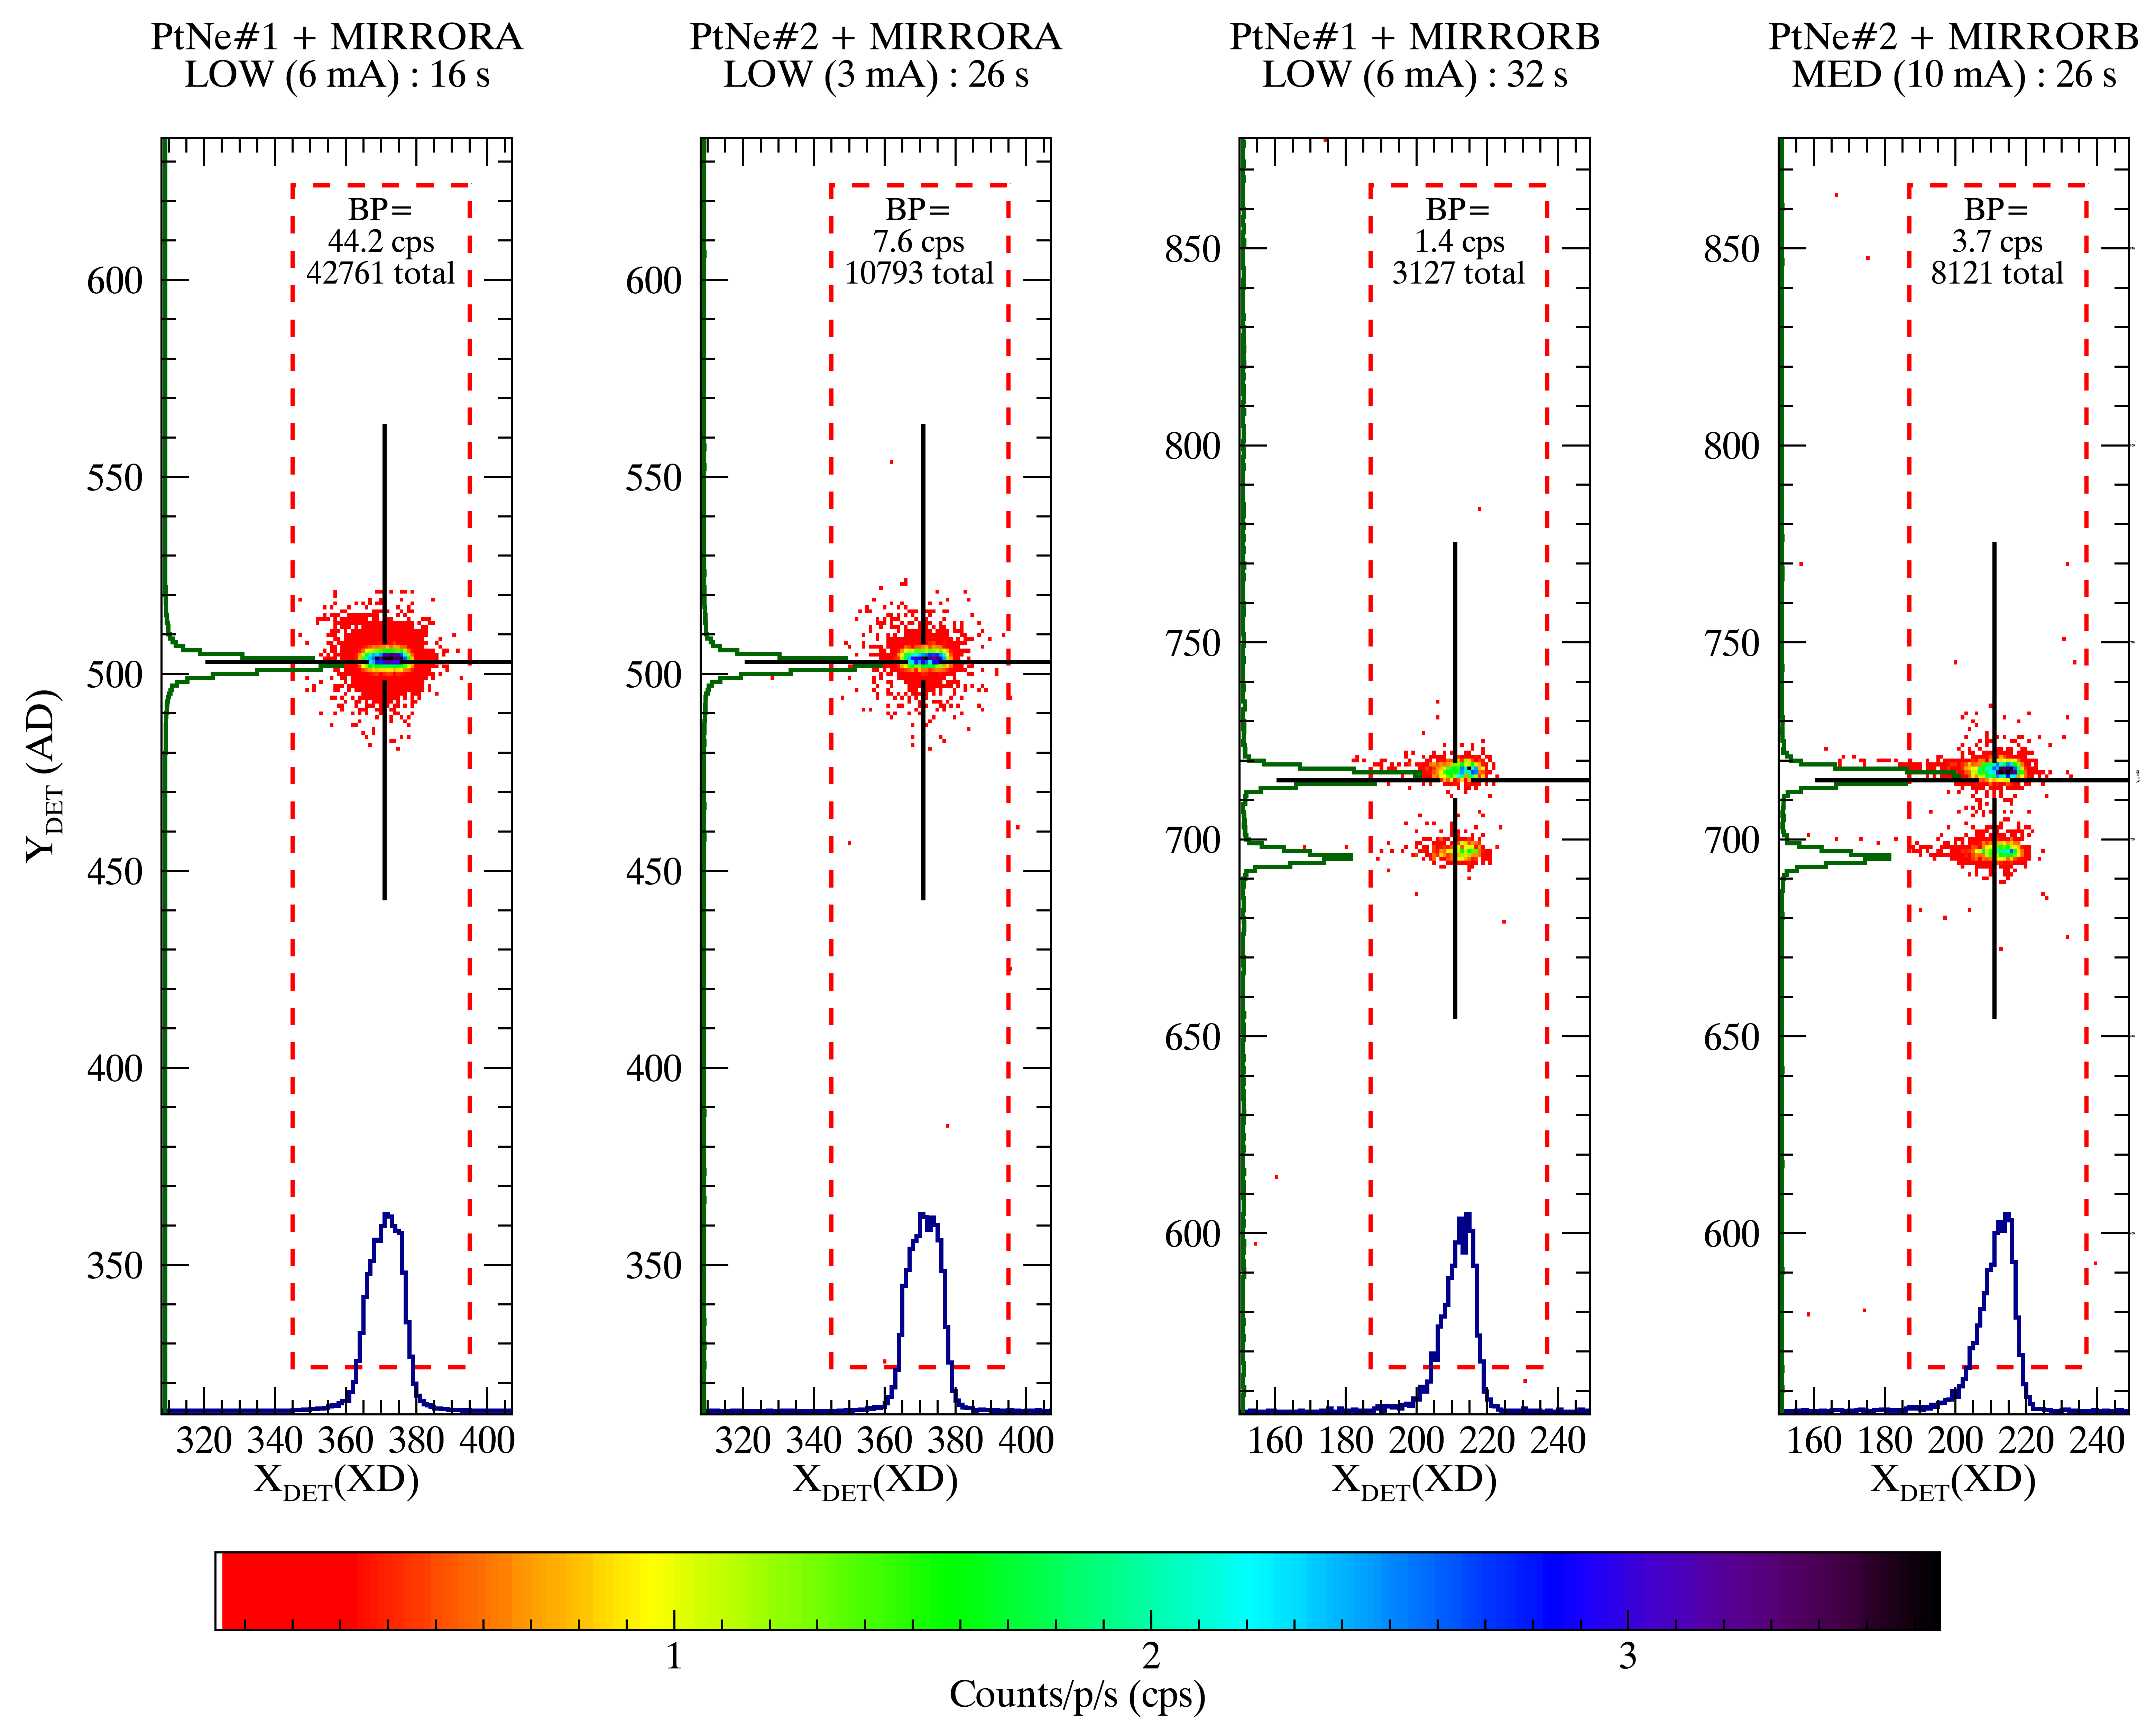
\includegraphics[width=\textwidth]{C24_14857_FP.png}
		\caption{These four panels show a ``family portrait'' of the available COS PtNe Lamp + MIRROR combinations possible with \tacq{IMAGE}. Panel titles give the lamp and mirror combination, along with the current setting (in milli-amps, mA) and the exposure times in this program.
		These images are in `detector' coordinates, as used on-board COS.
		The images show the observed counts/pixel/s (cps) as given by the colorbar on the bottom.
		The \textcolor{red}{red} dashed boxes show the Cycle~24 \tacq{IMAGE} WCA subarrays. At the top of the subarrays, text provides the count rate in the brightest pixel (BP) in units of counts per second per NUV MAMA pixel (cps).
		The \textcolor{blue}{blue} histogram on the bottom edge shows the cross-dispersion (XD) lamp profile in detector `X' coordinates, while
		the \textcolor{green}{green} histogram on the left edge shows the along-dispersion (AD) lamp profile in detector `Y' coordinates.
		The cross-hairs show the median location of the given configurations' lamp events within the TA subarray.
		PtNe\#2 lamp was used for all \tacq{IMAGE}s during Cycle~24, and was operated at LOW current (6~mA) for those using MIRRORA and MEDium current (10~mA) for those using MIRRORB.
		}
		\label{fig:FP}
		\vspace{1.3cm}
	\end{figure}

	\begin{table}[ht]
	\caption{HST COS Cycle~24 TA Monitoring (\pid{14857}) Results Summary}
	\def\arraystretch{1.25}
	\tabletypesize{\tiny}
	\footnotesize
	\begin{tabular}{ccccccc}
	\hline
	\hline
	ACQ & COS & Optical & Direction & Measured Offset\tablenotemark{b} & Requirement& Goal\\
	Mode & Channel & Configuration & AD or XD & mas\tablenotemark{a} & mas\tablenotemark{a} & mas\tablenotemark{a}\\
	\hline
	IMAGE	&	NUV	&	PSA+MIRRORA	&	AD	&	20$\pm$14	&	41--105	&	40\\
	IMAGE	&	NUV	&	PSA+MIRRORB	&	AD	&	10$\pm$14	&	41--105	&	40\\
	IMAGE	&	NUV	&	BOA+MIRRORA	&	AD	&	20$\pm$14	&	41--105	&	40\\
	IMAGE	&	NUV	&	BOA+MIRRORB	&	AD	&	15$\pm$14	&	41--105	&	40\\
	\hline
	IMAGE	&	NUV	&	PSA+MIRRORA	&	XD	&	75$\pm$14	&	300		&	100\\
	IMAGE	&	NUV	&	PSA+MIRRORB	&	XD	&	20$\pm$14	&	300		&	100\\
	IMAGE	&	NUV	&	BOA+MIRRORA	&	XD	&	95$\pm$14	&	300		&	100\\
	IMAGE	&	NUV	&	BOA+MIRRORB	&	XD	&	12$\pm$14	&	300		&	100\\
	PEAKXD	&	NUV	&	G185M		&	XD	&	 70$\pm$17		&	300		&	100\\
	PEAKXD	&	NUV	&	G225M		&	XD	&	 60$\pm$17		&	300		&	100\\
	PEAKXD	&	NUV	&	G285M		&	XD	&	 20$\pm$17		&	300		&	100\\
	PEAKXD	&	NUV	&	G230L		&	XD	&	 20$\pm$17		&	300		&	100\\
	PEAKXD	&	FUVA	&	G130M		&	XD	&	-30$\pm$71		&	300		&	100\\
	PEAKXD	&	FUVA	&	G160M		&	XD	&	-20$\pm$71		&	300		&	100\\
	PEAKXD	&	FUVA	&	G140L		&	XD	&	-170$\pm$71		&	300		&	100\\
	\hline
	\centering
	\tablenotetext{a}{1 mas = 1 milli-arcsecond.}
	\tablenotetext{b}{The quoted error bars are associated with a 0.5 uncertainty when measuring the integer WCA coordinate,
	and 1/3 of an NUV pixel when using the \tacq{IMAGE} checkbox centering algorithm. Added in quadrature, the approximate
	\tacq{IMAGE} measurement error is $\approx 0.6$ NUV pixels, or 14 mas.
	Each \tacq{PEAKXD}  WCA-to-SA measurement contains an error estimate of $\sqrt2 * 0.5 $ times the plate scale of the detector in use
	(one half pixel or digital-element uncertainty for each measurement of an integer quantity).
	For the NUV channel, this is 23.5 mas/p or $\sqrt2 * 0.5 * 23.5 = 17$ mas.
	For the FUV channel, this is $\approx \sqrt2 * 0.5 * 100 \approx 71$ mas.}
	\tablecomments{See \tamonISR{} for further details.}
	\end{tabular}
	\label{tab:exp}
	\end{table}
\clearpage
\vspace{-0.3cm}
\ssection{Conclusions.\label{sec:theend}}
\vspace{-0.3cm}
All COS TA modes were verified to be operating within the requirements during HST Cycle~24. All COS SIAF NUV (LP1) and FUV (LP3)
entries were determined to be accurate to the needs of COS operations, and all TA and science mode NUV (LP1) and FUV (LP3)
subarrays were determined to be correctly defined.
Spectroscopic TAs for all NUV gratings met all XD centering requirements.
All three FUV gratings indicated some level of Y-walk in the WCA-to-PSA offsets, and they were all in the -XD direction.
Only the G140L WCA-to-PSA offset indicates a potential Y-walk problem as its offset error ($0.17\arcsec$) is larger than the $0.1\arcsec$ XD centering goal and is $\approx 60\%$ of the XD centering requirement.
Continued monitoring of the LP3 FUV WCA-to-PSA offsets is warranted if LP3 FUV spectroscopic TAs are allowed beyond Cycle~24 to ensure they are properly centering targets in the XD.
Further details on HST Cycle 22 and 23 COS TA monitoring can be found in the annual summary ISRs; COS ISR 2016-09 (Cycle~22, HST PID 13972) and COS ISR 2017-18 (Cycle~23, \pid{14440}).
Complete details of program \pid{14857} and the complete Cycle 20--24 HST+COS TA monitoring program can be found in \tamonISR{}.

Further details about COS TA strategies can be found in COS ISR 2010-14 (Keyes, COS Target Acquisition Guidelines, Recommendations, and Interpretation) with detailed information about the on-orbit performance of early COS target acquisitions, including signal-to-noise requirements can be found in COS TIR 2010-14 (Penton, On-Orbit Target Acquisitions with HST+COS).
%%%%%%%%%
%Change History
%%%%%%%%
\vspace{-0.4cm}
%Put instrument, year, and ISR number
\ssectionstar{Change History for \thisISR{}}\label{sec:History}
\vspace{-0.3cm}
%Put publication date
%Version 0.5: 7-Dec-2017 Original Un-reviewed Document
Version 1.0: May 25, 2018 Original Document  % (reviewer = CO)
%%%%%%%%
%References
%%%%%%%%
\vspace{-0.6cm}
\ssectionstar{References}\label{sec:References}
\vspace{-0.4cm}
\noindent
Keyes, T., \& Penton, S., COS ISR 2010-14 (v1) (HST+COS Target Acquisition Guidelines, Recommendations, and Interpretation)\\
Penton, S., 2011, COS TIR 2010-03 (On-Orbit Target Acquisitions with HST+COS)\\
Penton, S., 2016, COS ISR 2016-09 (Cycle~22 HST+COS Target Acquisition Monitoring Summary (\pid{13972})\\
Penton, S., 2017, COS ISR 2017-18 (Cycle~23 HST+COS Target Acquisition Monitoring Summary (\pid{14440})\\
Penton, S., 2018, \tamonISR{} (Cycle 20--24 HST+COS Target Acquisition Monitoring)\\

%!!!!!!!!!!!!!!!!!!!!!!!!!!!!!!!!!!!!!!!!!!!!!!!!!!!!!!!!!!!!!!!!!!!!!!!!!!!!!!!!!!!!!!!!!!!!!!!!!!!!!!!!!!!!!!!!!!!!!!!!!!!!!!!!!!!!!!!!!!!!!!!!!!!!!!!!!!!!!!!!!!!!!!!!!!!!!!!!!!!!!!!!!!!!!!!!!!!!!!!!!!!!!!!!!!!!!!!!!!!!!!!!!!!!!!!!!!!!!!!!
%THIS SECTION NEEDS TO GO AFTER THE END OF THE FIRST PAGE AND BEFORE THE END OF THE SECOND PAGE
%Fill in Instrument, Year, and ISR Number and delete "newpage" immediately after this message
%!!!!!!!!!!!!!!!!!!!!!!!!!!!!!!!!!!!!!!!!!!!!!!!!!!!!!!!!!!!!!!!!!!!!!!!!!!!!!!!!!!!!!!!!!!!!!!!!!!!!!!!!!!!!!!!!!!!!!!!!!!!!!!!!!!!!!!!!!!!!!!!!!!!!!!!!!!!!!!!!!!!!!!!!!!!!!!!!!!!!!!!!!!!!!!!!!!!!!!!!!!!!!!!!!!!!!!!!!!!!!!!!!!!!!!!!!!!!!!
\lhead{}
\rhead{}
\cfoot{\rm {\hspace{-1.9cm} Instrument Science Report \thisISR{} Page \thepage}}
\end{document}
